\chapter{Conception et analyse du système}

    \section{Introduction}

        La simulation de milieux marins est quelque chose de connu dans le domaine de la robotique, et il en existe aujourd'hui déjà de nombreux~\cite{Manhaes_2016, bingham19toward, MARS, Rock}. Ces simulateurs proposent tous un modèle de flottabilité pour les objets à simuler, ce qui permet de pouvoir définir à la fois des bateaux et des robots sous-marins. Cela permet donc de pouvoir simuler le comportement des \gls{ROV}s dans l'eau. Ils proposent ensuite tous leur lot de spécificités qui permettent d'avoir des éléments supplémentaires dans notre simulation.
        
        \textsc{UUV Simulator}~\cite{Manhaes_2016} est probablement le plus connu d'entre eux. C'est un simulateur de \gls{ROV} comportant un certain nombre d'éléments d'environnements simulés, comme des mondes marins, du courant ou des ombilicaux par exemple. Il propose aussi la description d'un bon nombre de robots sous-marins commercialisés, et la communauté active partage les nouveaux modèles régulièrement.
        
        \textsc{Mars}~\cite{MARS} est un simulateur spécifique à des robot baptisés \textsc{Mars}. Il permet de supporter plusiieurs \gls{ROV}s et peut être commandé par \gls{ROS} ou bien en utilisant des sockets TCP.
        
        \textsc{Rock-Gazebo}~\cite{Rock} est un projet d'intégration de simulateur basé sur le moteur physique \gls{Gazebo} et sur le framework\footnote{Infrastructure logicielle facilitant le développement logiciel} \textsc{Robot Construction Kit}.
        
        Le simulateur \textsc{VRX}~\cite{bingham19toward} est un projet open-source de robotique marine dont un simulateur a été implémenté sur la base de \gls{Gazebo}. Il propose un ensemble d'environnement, de modèles et de plugin permettant la simulation de missions de vaisseaux de surface, avec notamment la possibilité de prendre en compte la présence de vagues et de vent à la surface.

        Ces simulateurs proposent tous des spécificités différentes et intéressantes. Cependant, notre application de simulation de \gls{ROV}s pour \textsc{Forssea Robotics} est assez contrainte. En effet, l'existance de composants spécifiques, comme la simulation du \gls{Latch} ainsi que la \gls{frameLBL} rendent l'adaptation de simulateurs déjà existants trop difficile. C'est pourquoi il est nécéssaire de réaliser notre propre simulateur.

    \section{Spécifications fonctionnelles}
        \label{sec:spec_fonc}

        Le système à concevoir doit permettre de simuler \gls{ROV}s de la société \textsc{Forssea Robotics} dans un environnement sous-marin. Le simulateur doit respecter un certain nombre de spécifications fonctionnelles qui délimitent les exigences requises par le système. La \textsc{Figure}~\ref{figure:pieuvre} complétée par la \textsc{Table}~\ref{table:specs} présentent les exigences du système.

        \begin{figure}[!htb]
            \centering
            \begin{tikzpicture}[scale=0.7, every node/.style={ellipse, align=center, scale=0.7}]
                \node[draw,minimum height=40pt, minimum width=100pt, fill=Lavender!80!pink!100] (S) at (0, 0) {Simulateur};
                \node[draw,minimum height=40pt, minimum width=100pt, fill=cyan!60!pink!70] (C0) at (0:5.5cm) {Middleware};
                \node[draw,minimum height=40pt, minimum width=100pt, fill=cyan!60!pink!70] (C1) at (48:3.5cm) {Robot};
                \node[draw,minimum height=40pt, minimum width=100pt, fill=cyan!60!pink!70] (C2) at (132:3.5cm) {Stockage};
                \node[draw,minimum height=40pt, minimum width=100pt, fill=cyan!60!pink!70] (C3) at (180:5.5cm) {Interface};
                \node[draw,minimum height=40pt, minimum width=100pt, fill=cyan!60!pink!70] (C4) at (228:3.5cm) {Capteur};
                \node[draw,minimum height=40pt, minimum width=100pt, fill=cyan!60!pink!70] (C5) at (312:3.5cm) {Environnement};
                
                \draw[blue!75, line width=0.8mm] (C1) -- (S) node[midway, fill=white]{FP1};
                \draw[orange!80, line width=0.8mm] (C0) -- (S) node[midway, fill=white]{FC3};
                \draw[orange!80, line width=0.8mm] (C3) -- (S) node[midway, fill=white]{FC1};
                \draw[orange!80, line width=0.8mm] (C5.90) -- (S.330) node[midway, fill=white]{FC2};
                \draw[orange!80, line width=0.8mm] (C2.320) to[bend left=70, in=158, out=60] node[fill=white, pos=0.25]{FC4} (C4.90);
                \draw[blue!75, line width=0.8mm] (C5.160) to[in=0, out=118] node[pos=0.25, fill=white]{FP2} (-0.3, -0.4) node (I){~} to[in=60, out=180] (C4.50);
            \end{tikzpicture}
            \caption{Diagramme pieuvre du simulateur}
            \label{figure:pieuvre}
        \end{figure}

        \begin{table}[!htb]
            \centering
            \begin{adjustbox}{max width=\textwidth}
                \begin{tabularx}{\textwidth}{|lX|}
                    \hline
                    \cellcolor{gray!25}\textbf{id} & \cellcolor{gray!25} \textbf{Fonction} \\
                    \hline \hline
                    \cellcolor{blue!30}\textbf{FP1}&\cellcolor{blue!25} Le système doit avoir un comportement proche du robot réel. \\
                    \hline
                    \cellcolor{gray!10}FP1.1& Le système doit utiliser des dimensions semblables au robot réel. \\
                    \hline
                    \cellcolor{gray!10}FP1.2& Le système doit avoir des masses et des inerties semblables au robot réel. \\
                    \hline
                    \cellcolor{gray!10}FP1.3& Le système doit avoir les mêmes degrès de liberté que le robot réel. \\
                    \hline
                    \cellcolor{gray!10}FP1.4& Le système doit avoir les mêmes actionneurs que le robot réel. \\
            
                    \hline \hline
            
                    \cellcolor{blue!30}\textbf{FP2}&\cellcolor{blue!25} Le système doit simuler le comportement de capteurs afin d'acquérir des informations sur l'environnement de simulation. \\
                    \hline
                    \cellcolor{gray!10}FP2.1& Le système doit simuler les capteurs suivants :
                    \begin{compactitem}[\textbullet]
                        \item Camera RGB
                        \item Lidar 3D
                        \item Sonar
                    \end{compactitem} \\ [-\normalbaselineskip]
                    \hline
                    \cellcolor{gray!10}FP2.2& Les mesures des capteurs doivent être bruitées numériquement afin d'être le plus proche de capteurs réels. \\
                    \hline
            
                    \hline \hline
            
                    \cellcolor{orange!40}\textbf{FC1} &\cellcolor{orange!30} Le système doit être interfaceable avec l'implémentation logicielle afin de pouvoir tester le comportement du robot. \\
                    \hline
                    \cellcolor{gray!10}FC1.1& Le système doit interpréter les commandes actionneurs de la partie implémentation logicielle. \\
                    \hline
                    \cellcolor{gray!10}FC1.2& Le système doit communiquer son état à l'implémentation logicielle.\\
                    \hline
            
                    \hline \hline
            
                    \cellcolor{orange!40}\textbf{FC2}&\cellcolor{orange!30} Le système doit pouvoir évoluer dans différents environnements simulés. \\
                    \hline
                    \cellcolor{gray!10}FC2.1& Le système doit pouvoir évoluer dans un monde vide. \\
                    \hline
                    \cellcolor{gray!10}FC2.2& Le système doit pouvoir évoluer dans une vigne ayant une largeur paramétrable. \\
                    \hline
                    \cellcolor{gray!10}FC2.3& Le système doit pouvoir entrer en collision avec les objets solides de l'environnement de simulation. \\
            
                    \hline \hline
            
                    \cellcolor{orange!40}\textbf{FC3}&\cellcolor{orange!30} Le système doit être compatible avec le \textsc{Middleware} choisi pour l'iplémentation logicielle. \\
                    \hline
            
                    \hline \hline
            
                    \cellcolor{orange!40}\textbf{FC4}&\cellcolor{orange!30} Le système doit pouvoir enregistrer les données des capteurs pour être analysées ultérieurement. \\
                    \hline
                    \cellcolor{gray!10}FC4.1& Le système doit utiliser des messages standard pour le transit de données des capteurs. \\
                    \hline
                \end{tabularx}
            \end{adjustbox}
            \caption{Spécifications fonctionnelles du simulateur}
            \label{table:specs}
        \end{table}    

    \section{Spécifications techniques}

        Pour remplir les différentes spécifications fonctionnelles présentées dans la \textsc{Section}~\ref{sec:spec_fonc}, nous allons définir un certain nombre de spécifications techniques. Ces dernières vont proposer les outils et les différents critères permettant de remplir les exigences attendues.

    \section{Logiciel de simulation}

        En outre, l'étude de l'existant nous aura au moins permis de se rendre compte que \gls{Gazebo}~\cite{Koenig-gazebo} est largement utilisé dans le domaine de la simulation sous-marine, mais aussi plus largement dans la simulation robotique. \gls{Gazebo} est un logiciel de simulation multi-physique open-source\footnote{Code communautaire ouvert libre de redistribution et d'accès}. Il est aujourd'hui développé par la communauté \gls{OpenRobotics}. Il présente l'avantage de pouvoir communiquer avec \gls{ROS}, ce qui est une exigence importante de notre simulateur, car il doit permettre de tester l'implémentation logicielle des robots. La description des robots se fait en utilisant le language \gls{SDF}\footnote{\url{http://sdformat.org/}}, et il est possible de décrire le comportement complexe d'un composant en implémentant un \gls{Plugin}.

    \section{Architecture logicielle}

        L'exigence principale du simulateur étant de s'interfacer parfaitement avec le reste de l'implémentation logicielle, il est nécéssaire de définir une architecture logicielle permettant de communiquer à la fois avec les \gls{ROV}s réels et simulés. \gls{ROS2Control}~\cite{ros_control} est un framework permettant de faire communiquer des contrôleurs et des drivers ensemble. L'avantage est de pouvoir changer à chaud de contôleurs de manière consistante, sans temps mort durant lesquels le robot ne serait pas commandé.

        \begin{figure}[!htb]
            \centering
            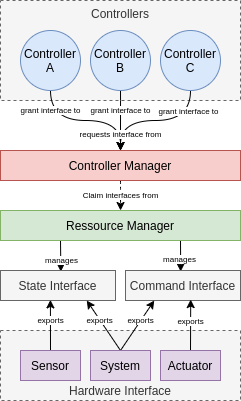
\includegraphics{imgs/ros2_control.pdf}
            \caption{Architecture logicielle avec \gls{ROS2Control}}
            \label{fig:ros2_control}
        \end{figure}

        La \textsc{Figure}~\ref{fig:ros2_control} nous montre l'architecture logicielle de \gls{ROS2Control}. Ce framework va instancier un \gls{ControllerManager} qui va s'occuper de charger les contrôleurs qui seront utilisés dans le robot, des \gls{HardwareInterface} qui sont les interfaces qui vont communiquer avec les composants et un \gls{RessourceManager} qui va faire transiter les données entre les contrôleurs et les composants. L'\gls{HardwareInterface} peut être réelle ou simulées, c'est-à dire qu'elle peut communiquer avec des vrai composants ou des composants simulés. L'idée est de crée une \gls{HardwareInterface} proposant les mêmes interfaces que celle implémentée pour les composants réels. Ainsi on peut utiliser les mêmes algorithmes de contrôle de manière totalement transparente sur les composant réels et les composants simulés.
